\documentclass{article}
\usepackage[utf8]{inputenc}
\usepackage{tikz}
\usetikzlibrary{calc, trees, positioning, arrows, fit, shapes}
\usepackage{amsmath}
\usepackage{amssymb}

\newcommand*{\blackboard}[1]{\mathbb{#1}}%

\pgfkeys{/tikz/.cd,
     num vertex/.initial=4,
     num vertex/.get=\vertices,
     num vertex/.store in=\vertices,
     circle radius/.initial=3,
     circle radius/.get=\circleradius,
     circle radius/.store in=\circleradius,
     shift angle/.initial=0,
     shift angle/.get=\shiftangle,
     shift angle/.store in=\shiftangle, 
     at pos/.initial={(0,0)},
     at pos/.get=\position,
     at pos/.store in=\position,
     vertex radius/.initial=1.5pt,
     vertex radius/.get=\vertexradius,
     vertex radius/.store in=\vertexradius,
}

% that's just an alias for \node
\makeatletter
\def\drawvertices{\tikz@path@overlay{node}}
\makeatother   

\pgfkeys{/tikz/circumference with labels/.code={
        \pgfmathsetmacro\halfcircleradius{\circleradius/2}
        \draw \position circle (\halfcircleradius cm) node[regular polygon, regular polygon sides=\vertices, minimum size=\circleradius cm, draw=none, name={vertex set}] {};
        \foreach \textlabel/\circlecolor [count=\x] in {#1}{
            \node[draw,circle, inner sep=\vertexradius,black, fill=\circlecolor] at (vertex set.corner \x) {};
            \pgfmathparse{\shiftangle-360*(\x-1)/ \vertices}
            \node at ($(vertex set)+(\pgfmathresult:\halfcircleradius)$)[label={[font=\small]\pgfmathresult:$\textlabel$}]{};
        }
    }
}

\pgfkeys{/tikz/circumference with labels in order/.code={
        \pgfmathsetmacro\halfcircleradius{\circleradius/2}
        \draw \position circle (\halfcircleradius cm) node[regular polygon, regular polygon sides=\vertices, minimum size=\circleradius cm, draw=none, name={vertex set}] {};
        \foreach \circlecolor [count=\x] in {#1}{
            \node[draw,circle, inner sep=\vertexradius,black, fill=\circlecolor] at (vertex set.corner \x) {};
            \pgfmathparse{\shiftangle-360*(\x-1)/ \vertices}
            \node at ($(vertex set)+(\pgfmathresult:\halfcircleradius)$)[label={[font=\small]\pgfmathresult:$\x$}]{};
        }
    }
}  

\title{Group Theory}
\author{Daniel Long}
\date{May 2021}

\begin{document}

\maketitle

\tableofcontents

\section{Fundamentals of a Group}

\subsection{What is a Group?}

Groups are number systems with a set of numbers/symbols and defined operations, for example the set of integers:
\[ \mathbb{Z} = \{ 0, +1, -1, +2, -2, ... \} \]
can be defined with the operation of addition (an example of a composition law) and remain closed.

Another group could be:
\[ G= \{ \phi, \Phi, D \} \]
with the a general composition law of
\[ x \circ y \]
sometimes written as \( x + y \), \( x \times y \), \( xy \)

\subsection{What is a Composition Law?}

Composition laws can be defined with a composition table:

\begin{center}
\begin{tabular}{ |c|c c c| } 
 \hline
 $\circ$ & $\phi$ & $\Phi$ & D \\
 \hline
 $\phi$ & $\phi$ $\circ$ $\phi$ & $\phi$ $\circ$ $\Phi$ & $\phi$ $\circ$ D \\
 $\Phi$ & $\Phi$ $\circ$ $\phi$ & $\Phi$ $\circ$ $\Phi$ & $\Phi$ $\circ$ D \\
 D & D $\circ$ $\phi$ & D $\circ$ $\Phi$ & D $\circ$ D \\
 \hline
\end{tabular}
\end{center}

The composition table must obey the following axioms:
\begin{enumerate}
 \item Closure - All composition products exist within the group
 \item Identity - \( e \circ g = g \circ e = g \)
 \item Associativity - \((x \circ y) \circ z = x \circ (y \circ z)\)
 \item Inverses - \(\forall g \in G \: \exists \: g^{-1} \:  s.t. \: g \circ g^{-1} = g^{-1} \circ g = e\)
\end{enumerate}

\subsection{Associativity}

Building a group that obeys associativity can be tricky, fortunately there is a method for this problem. Start by defining the set of permutations / bijective mappings for the set \( \{ a, b \} \) such that:

\begin{center}
 \centering
 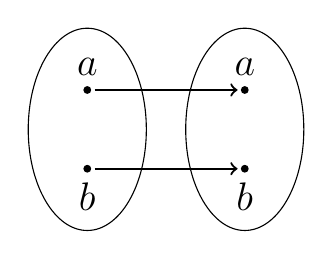
\begin{tikzpicture}[ele/.style={fill=black, circle, minimum width=.1pt, inner sep=1pt},every fit/.style={ellipse, draw, inner sep=10pt},every label/.append style={font=\Large}]
  \node[ele, label = above:$a$] (a1) at (0,4) {};
  \node[ele, label = below:$b$] (a2) at (0,3) {};

  \node[ele, label = above:$a$] (b1) at (2,4) {};
  \node[ele, label = below:$b$] (b2) at (2,3) {};

  \node[draw, fit = (a1) (a2), minimum width = 1.5cm] {};
  \node[draw, fit = (b1) (b2), minimum width = 1.5cm] {};  
  \draw[->, thick, shorten <= 1pt, shorten >= 1pt] (a1) -- (b1);
  \draw[->, thick, shorten <= 1pt, shorten >= 1pt] (a2) -- (b2);
 \end{tikzpicture}
\end{center}

\centerline{\LARGE \( i \)}
\vspace{5mm}

\begin{center}
 \centering
 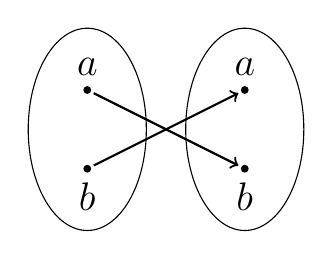
\begin{tikzpicture}[ele/.style={fill=black, circle, minimum width=.1pt, inner sep=1pt},every fit/.style={ellipse, draw, inner sep=10pt},every label/.append style={font=\Large}]
  \node[ele, label = above:$a$] (a1) at (0,4) {};
  \node[ele, label = below:$b$] (a2) at (0,3) {};

  \node[ele, label = above:$a$] (b1) at (2,4) {};
  \node[ele, label = below:$b$] (b2) at (2,3) {};

  \node[draw, fit = (a1) (a2), minimum width = 1.5cm] {};
  \node[draw, fit = (b1) (b2), minimum width = 1.5cm] {};
  \draw[->, thick, shorten <= 1pt, shorten >= 1pt] (a1) -- (b2);
  \draw[->, thick, shorten <= 1pt, shorten >= 1pt] (a2) -- (b1);
 \end{tikzpicture}
\end{center}

\centerline{\LARGE \( \tau \)}
\vspace{5mm}

With both of these mappings defined we can then define a group with the group \( G = {i, \tau} \) with the following composition table:

\begin{center}
\begin{tabular}{ |c|c c| } 
 \hline
 $\circ$ & i & $\tau$ \\
 \hline
 i & i & $\tau$ \\
 $\tau$ & $\tau$ & i \\
 \hline
\end{tabular}
\end{center}

The compositions can be seen in the following diagrams:

\vspace{5mm}

\begin{center}
 \centering
 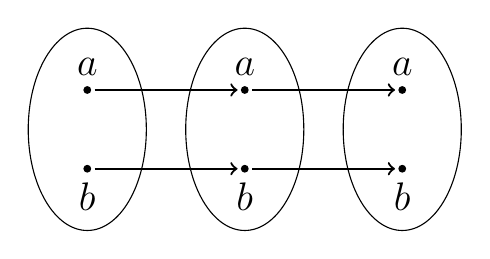
\begin{tikzpicture}[ele/.style={fill=black, circle, minimum width=.1pt, inner sep=1pt},every fit/.style={ellipse, draw, inner sep=10pt},every label/.append style={font=\Large}]
  \node[ele, label = above:$a$] (a1) at (0,4) {};
  \node[ele, label = below:$b$] (a2) at (0,3) {};

  \node[ele, label = above:$a$] (b1) at (2,4) {};
  \node[ele, label = below:$b$] (b2) at (2,3) {};

  \node[ele, label = above:$a$] (c1) at (4,4) {};
  \node[ele, label = below:$b$] (c2) at (4,3) {};

  \node[draw, fit = (a1) (a2), minimum width = 1.5cm] {};
  \node[draw, fit = (b1) (b2), minimum width = 1.5cm] {};
  \node[draw, fit = (c1) (c2), minimum width = 1.5cm] {};
  \draw[->, thick, shorten <= 1pt, shorten >= 1pt] (a1) -- (b1);
  \draw[->, thick, shorten <= 1pt, shorten >= 1pt] (a2) -- (b2);
  \draw[->, thick, shorten <= 1pt, shorten >= 1pt] (b1) -- (c1);
  \draw[->, thick, shorten <= 1pt, shorten >= 1pt] (b2) -- (c2);
 \end{tikzpicture}
\end{center}

\centerline{\LARGE \( i \circ i \)}
\vspace{5mm}

\begin{center}
 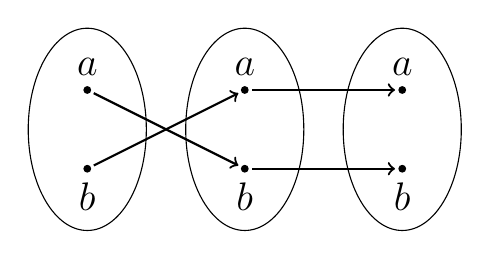
\begin{tikzpicture}[ele/.style={fill=black, circle, minimum width=.1pt, inner sep=1pt},every fit/.style={ellipse, draw, inner sep=10pt},every label/.append style={font=\Large}]
  \node[ele, label = above:$a$] (a1) at (0,4) {};
  \node[ele, label = below:$b$] (a2) at (0,3) {};

  \node[ele, label = above:$a$] (b1) at (2,4) {};
  \node[ele, label = below:$b$] (b2) at (2,3) {};

  \node[ele, label = above:$a$] (c1) at (4,4) {};
  \node[ele, label = below:$b$] (c2) at (4,3) {};

  \node[draw, fit = (a1) (a2), minimum width = 1.5cm] {};
  \node[draw, fit = (b1) (b2), minimum width = 1.5cm] {};
  \node[draw, fit = (c1) (c2), minimum width = 1.5cm] {};
  \draw[->, thick, shorten <= 1pt, shorten >= 1pt] (a1) -- (b2);
  \draw[->, thick, shorten <= 1pt, shorten >= 1pt] (a2) -- (b1);
  \draw[->, thick, shorten <= 1pt, shorten >= 1pt] (b1) -- (c1);
  \draw[->, thick, shorten <= 1pt, shorten >= 1pt] (b2) -- (c2);
 \end{tikzpicture}
\end{center}

\centerline{\LARGE \( i \circ \tau \)}
\vspace{5mm}

This approach represents compositions as compositions of set permutations. Making sure that the original set's compositions obey the following composition laws of the set permutations will result in associativity holding true.

Applying this perspective to the group of real integers \( Z \) we can view the number line as a sequence of points and the integers as mappings or permutations between those sequences. For example 0 can be visualised as the following mapping:

\begin{center}
 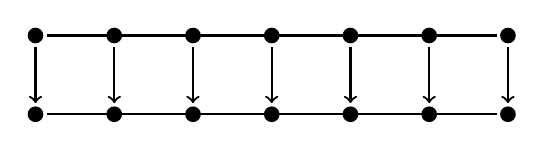
\begin{tikzpicture}[ele/.style={fill=black, circle, minimum width=.3pt, inner sep=2pt}]
  \node[ele] (a1) at (0,4) {};
  \node[ele] (a2) at (1,4) {};
  \node[ele] (a3) at (2,4) {};
  \node[ele] (a4) at (3,4) {};
  \node[ele] (a5) at (4,4) {};
  \node[ele] (a6) at (5,4) {};
  \node[ele] (a7) at (6,4) {};
  
  \node[ele] (b1) at (0,3) {};
  \node[ele] (b2) at (1,3) {};
  \node[ele] (b3) at (2,3) {};
  \node[ele] (b4) at (3,3) {};
  \node[ele] (b5) at (4,3) {};
  \node[ele] (b6) at (5,3) {};
  \node[ele] (b7) at (6,3) {};
  
  \draw[-, thick, shorten <= 1pt, shorten >= 1pt] (a1) -- (a7);
  \draw[-, thick, shorten <= 1pt, shorten >= 1pt] (b1) -- (b7);
  
  \draw[->, thick, shorten <= 1pt, shorten >= 1pt] (a1) -- (b1);
  \draw[->, thick, shorten <= 1pt, shorten >= 1pt] (a2) -- (b2);
  \draw[->, thick, shorten <= 1pt, shorten >= 1pt] (a3) -- (b3);
  \draw[->, thick, shorten <= 1pt, shorten >= 1pt] (a4) -- (b4);
  \draw[->, thick, shorten <= 1pt, shorten >= 1pt] (a5) -- (b5);
  \draw[->, thick, shorten <= 1pt, shorten >= 1pt] (a6) -- (b6);
  \draw[->, thick, shorten <= 1pt, shorten >= 1pt] (a7) -- (b7);
 \end{tikzpicture}
\end{center}

\centerline{\LARGE 0}
\vspace{5mm}

And +1 can be visualised as:

\begin{center}
 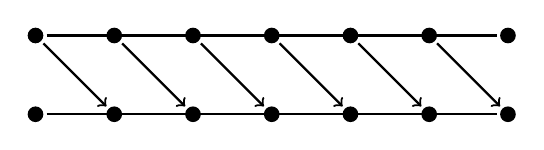
\begin{tikzpicture}[ele/.style={fill=black, circle, minimum width=.3pt, inner sep=2pt}]
  \node[ele] (a1) at (0,4) {};
  \node[ele] (a2) at (1,4) {};
  \node[ele] (a3) at (2,4) {};
  \node[ele] (a4) at (3,4) {};
  \node[ele] (a5) at (4,4) {};
  \node[ele] (a6) at (5,4) {};
  \node[ele] (a7) at (6,4) {};
  
  \node[ele] (b1) at (0,3) {};
  \node[ele] (b2) at (1,3) {};
  \node[ele] (b3) at (2,3) {};
  \node[ele] (b4) at (3,3) {};
  \node[ele] (b5) at (4,3) {};
  \node[ele] (b6) at (5,3) {};
  \node[ele] (b7) at (6,3) {};
  
  \draw[-, thick, shorten <= 1pt, shorten >= 1pt] (a1) -- (a7);
  \draw[-, thick, shorten <= 1pt, shorten >= 1pt] (b1) -- (b7);
  
  \draw[->, thick, shorten <= 1pt, shorten >= 1pt] (a1) -- (b2);
  \draw[->, thick, shorten <= 1pt, shorten >= 1pt] (a2) -- (b3);
  \draw[->, thick, shorten <= 1pt, shorten >= 1pt] (a3) -- (b4);
  \draw[->, thick, shorten <= 1pt, shorten >= 1pt] (a4) -- (b5);
  \draw[->, thick, shorten <= 1pt, shorten >= 1pt] (a5) -- (b6);
  \draw[->, thick, shorten <= 1pt, shorten >= 1pt] (a6) -- (b7);
 \end{tikzpicture}
\end{center}

\centerline{\LARGE +1}
\vspace{5mm}


\subsection{Identity}

An identity is required for a valid group, it is often represented with \( e, i, 0, 1 \). The identity is defined to compose with any other group elements to produce that group element. Ie it holds that:

\[ e \circ g = g \circ e = g \]

\section{Symmetric Groups}

A symmetric group is denoted as \(S_{n}\) where \(n \in \blackboard{N}\). The group is the number of set permutations within the set of natural numbers less than or equal to $n$. The order of a group is the number of elements in the group, which follows the law:

\[|S_{n}| = n!\]

\subsection{$S_{1}$}

\[ S_{1} = \{i\} \]

with the composition table:

\begin{center}
\begin{tabular}{ |c|c| } 
 \hline
 $\circ$ & $i$ \\
 \hline
 $i$ & $i$ \\
 \hline
\end{tabular}
\end{center}

which corresponds to the following set permutation:

\begin{center}
 \centering
 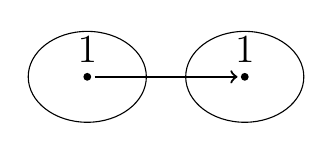
\begin{tikzpicture}[ele/.style={fill=black, circle, minimum width=.1pt, inner sep=1pt},every fit/.style={ellipse, draw, inner sep=10pt},every label/.append style={font=\Large}]
  \node[ele, label = above:$1$] (a1) at (0,4) {};

  \node[ele, label = above:$1$] (b1) at (2,4) {};

  \node[draw, fit = (a1), minimum width = 1.5cm] {};
  \node[draw, fit = (b1), minimum width = 1.5cm] {};
  \draw[->, thick, shorten <= 1pt, shorten >= 1pt] (a1) -- (b1);
 \end{tikzpicture}
\end{center}

\centerline{\LARGE \( i \)}
\vspace{5mm}

\subsection{$S_{2}$}

\[ S_{2} = \{i, \tau\} \]

with the following composition table:

\begin{center}
\begin{tabular}{ |c|c c| } 
 \hline
 $\circ$ & i & $\tau$ \\
 \hline
 i & i & $\tau$ \\
 $\tau$ & $\tau$ & i \\
 \hline
\end{tabular}
\end{center}

which corresponds to the following set permutations:

\begin{center}
 \centering
 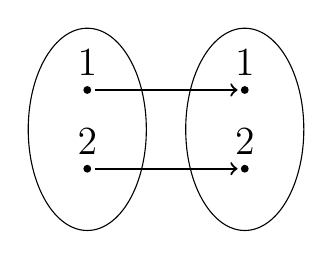
\begin{tikzpicture}[ele/.style={fill=black, circle, minimum width=.1pt, inner sep=1pt},every fit/.style={ellipse, draw, inner sep=10pt},every label/.append style={font=\Large}]
  \node[ele, label = above:$1$] (a1) at (0,4) {};
  \node[ele, label = above:$2$] (a2) at (0,3) {};

  \node[ele, label = above:$1$] (b1) at (2,4) {};
  \node[ele, label = above:$2$] (b2) at (2,3) {};

  \node[draw, fit = (a1) (a2), minimum width = 1.5cm] {};
  \node[draw, fit = (b1) (b2), minimum width = 1.5cm] {};
  \draw[->, thick, shorten <= 1pt, shorten >= 1pt] (a1) -- (b1);
  \draw[->, thick, shorten <= 1pt, shorten >= 1pt] (a2) -- (b2);
 \end{tikzpicture}
\end{center}

\centerline{\LARGE \( i \)}
\vspace{5mm}

\begin{center}
 \centering
 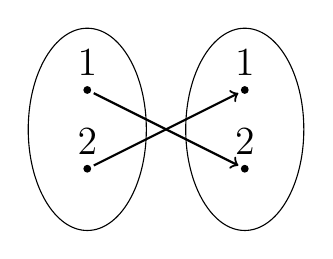
\begin{tikzpicture}[ele/.style={fill=black, circle, minimum width=.1pt, inner sep=1pt},every fit/.style={ellipse, draw, inner sep=10pt},every label/.append style={font=\Large}]
  \node[ele, label = above:$1$] (a1) at (0,4) {};
  \node[ele, label = above:$2$] (a2) at (0,3) {};

  \node[ele, label = above:$1$] (b1) at (2,4) {};
  \node[ele, label = above:$2$] (b2) at (2,3) {};

  \node[draw, fit = (a1) (a2), minimum width = 1.5cm] {};
  \node[draw, fit = (b1) (b2), minimum width = 1.5cm] {};
  \draw[->, thick, shorten <= 1pt, shorten >= 1pt] (a1) -- (b2);
  \draw[->, thick, shorten <= 1pt, shorten >= 1pt] (a2) -- (b1);
 \end{tikzpicture}
\end{center}

\centerline{\LARGE \( \tau \)}
\vspace{5mm}

\subsection{$S_{3}$}

\[ S_{3} = \{i, \tau_{12}, \tau_{13}, \tau_{23}, \sigma, \sigma^{2}\} \]

with the following composition table:

\begin{center}
\begin{tabular}{ |c|c c c c c c| } 
 \hline
 $\circ$ & i & $\tau_{12}$ & $\tau_{13}$ & $\tau_{23}$ & $\sigma$ & $\sigma^{2}$ \\
 \hline
 i & i & $\tau_{12}$ & $\tau_{13}$ & $\tau_{23}$ & $\sigma$ & $\sigma^{2}$ \\
 $\tau_{12}$ & $\tau_{12}$ & i & $\sigma$ & $\sigma^{2}$ & $\tau_{13}$ & $\tau_{23}$ \\
 $\tau_{13}$ & $\tau_{13}$ & $\sigma^{2}$ & i & $\sigma$ & $\tau_{23}$ & $\tau_{12}$ \\
 $\tau_{23}$ & $\tau_{23}$ & $\sigma$ & $\sigma^{2}$ & i & $\tau_{12}$ & $\tau_{13}$ \\
 $\sigma$ & $\sigma$  & $\tau_{23}$ & $\tau_{12}$ & $\tau_{13}$ & $\sigma^{2}$ & i \\
 $\sigma^{2}$ & $\sigma^{2}$ & $\tau_{13}$ & $\tau_{23}$ & $\tau_{12}$ & i & $\sigma$ \\
 \hline
\end{tabular}
\end{center}

\textit{Note: this composition table is non-symmetric, therefore it is non-commutative.}

\vspace{5mm}

as it corresponds to the following set permutations:

\begin{center}
 \centering
 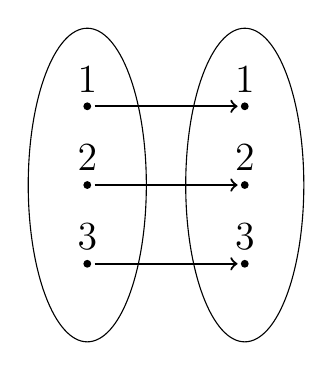
\begin{tikzpicture}[ele/.style={fill=black, circle, minimum width=.1pt, inner sep=1pt},every fit/.style={ellipse, draw, inner sep=10pt},every label/.append style={font=\Large}]
  \node[ele, label = above:$1$] (a1) at (0,4) {};
  \node[ele, label = above:$2$] (a2) at (0,3) {};
  \node[ele, label = above:$3$] (a3) at (0,2) {};

  \node[ele, label = above:$1$] (b1) at (2,4) {};
  \node[ele, label = above:$2$] (b2) at (2,3) {};
  \node[ele, label = above:$3$] (b3) at (2,2) {};

  \node[draw, fit = (a1) (a2) (a3), minimum width = 1.5cm] {};
  \node[draw, fit = (b1) (b2) (b3), minimum width = 1.5cm] {};
 
  \draw[->, thick, shorten <= 1pt, shorten >= 1pt] (a1) -- (b1);
  \draw[->, thick, shorten <= 1pt, shorten >= 1pt] (a2) -- (b2);
  \draw[->, thick, shorten <= 1pt, shorten >= 1pt] (a3) -- (b3);
 \end{tikzpicture}
\end{center}

\centerline{\LARGE \( i \)}
\vspace{5mm}

\begin{center}
 \centering
 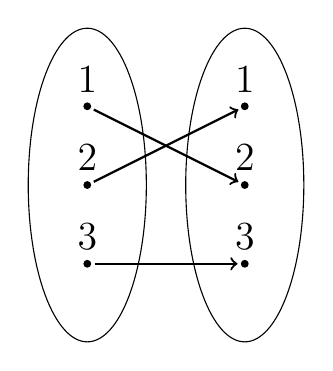
\begin{tikzpicture}[ele/.style={fill=black, circle, minimum width=.1pt, inner sep=1pt},every fit/.style={ellipse, draw, inner sep=10pt},every label/.append style={font=\Large}]
  \node[ele, label = above:$1$] (a1) at (0,4) {};
  \node[ele, label = above:$2$] (a2) at (0,3) {};
  \node[ele, label = above:$3$] (a3) at (0,2) {};

  \node[ele, label = above:$1$] (b1) at (2,4) {};
  \node[ele, label = above:$2$] (b2) at (2,3) {};
  \node[ele, label = above:$3$] (b3) at (2,2) {};

  \node[draw, fit = (a1) (a2) (a3), minimum width = 1.5cm] {};
  \node[draw, fit = (b1) (b2) (b3), minimum width = 1.5cm] {};
 
  \draw[->, thick, shorten <= 1pt, shorten >= 1pt] (a1) -- (b2);
  \draw[->, thick, shorten <= 1pt, shorten >= 1pt] (a2) -- (b1);
  \draw[->, thick, shorten <= 1pt, shorten >= 1pt] (a3) -- (b3);
 \end{tikzpicture}
\end{center}

\centerline{\LARGE \( \tau_{12} \)}
\vspace{5mm}

\begin{center}
 \centering
 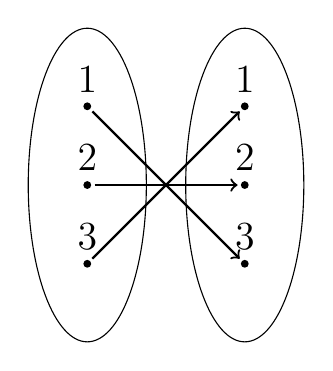
\begin{tikzpicture}[ele/.style={fill=black, circle, minimum width=.1pt, inner sep=1pt},every fit/.style={ellipse, draw, inner sep=10pt},every label/.append style={font=\Large}]
  \node[ele, label = above:$1$] (a1) at (0,4) {};
  \node[ele, label = above:$2$] (a2) at (0,3) {};
  \node[ele, label = above:$3$] (a3) at (0,2) {};

  \node[ele, label = above:$1$] (b1) at (2,4) {};
  \node[ele, label = above:$2$] (b2) at (2,3) {};
  \node[ele, label = above:$3$] (b3) at (2,2) {};

  \node[draw, fit = (a1) (a2) (a3), minimum width = 1.5cm] {};
  \node[draw, fit = (b1) (b2) (b3), minimum width = 1.5cm] {};
 
  \draw[->, thick, shorten <= 1pt, shorten >= 1pt] (a1) -- (b3);
  \draw[->, thick, shorten <= 1pt, shorten >= 1pt] (a2) -- (b2);
  \draw[->, thick, shorten <= 1pt, shorten >= 1pt] (a3) -- (b1);
 \end{tikzpicture}
\end{center}

\centerline{\LARGE \( \tau_{13} \)}
\vspace{5mm}

\begin{center}
 \centering
 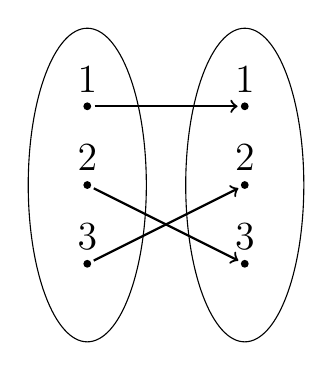
\begin{tikzpicture}[ele/.style={fill=black, circle, minimum width=.1pt, inner sep=1pt},every fit/.style={ellipse, draw, inner sep=10pt},every label/.append style={font=\Large}]
  \node[ele, label = above:$1$] (a1) at (0,4) {};
  \node[ele, label = above:$2$] (a2) at (0,3) {};
  \node[ele, label = above:$3$] (a3) at (0,2) {};

  \node[ele, label = above:$1$] (b1) at (2,4) {};
  \node[ele, label = above:$2$] (b2) at (2,3) {};
  \node[ele, label = above:$3$] (b3) at (2,2) {};

  \node[draw, fit = (a1) (a2) (a3), minimum width = 1.5cm] {};
  \node[draw, fit = (b1) (b2) (b3), minimum width = 1.5cm] {};
 
  \draw[->, thick, shorten <= 1pt, shorten >= 1pt] (a1) -- (b1);
  \draw[->, thick, shorten <= 1pt, shorten >= 1pt] (a2) -- (b3);
  \draw[->, thick, shorten <= 1pt, shorten >= 1pt] (a3) -- (b2);
 \end{tikzpicture}
\end{center}

\centerline{\LARGE \( \tau_{23} \)}
\vspace{5mm}

\begin{center}
 \centering
 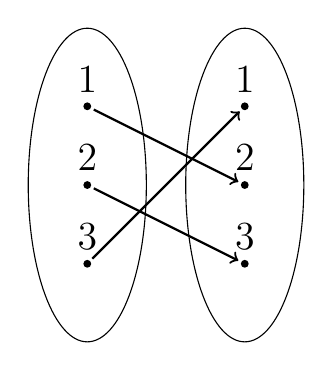
\begin{tikzpicture}[ele/.style={fill=black, circle, minimum width=.1pt, inner sep=1pt},every fit/.style={ellipse, draw, inner sep=10pt},every label/.append style={font=\Large}]
  \node[ele, label = above:$1$] (a1) at (0,4) {};
  \node[ele, label = above:$2$] (a2) at (0,3) {};
  \node[ele, label = above:$3$] (a3) at (0,2) {};

  \node[ele, label = above:$1$] (b1) at (2,4) {};
  \node[ele, label = above:$2$] (b2) at (2,3) {};
  \node[ele, label = above:$3$] (b3) at (2,2) {};

  \node[draw, fit = (a1) (a2) (a3), minimum width = 1.5cm] {};
  \node[draw, fit = (b1) (b2) (b3), minimum width = 1.5cm] {};
 
  \draw[->, thick, shorten <= 1pt, shorten >= 1pt] (a1) -- (b2);
  \draw[->, thick, shorten <= 1pt, shorten >= 1pt] (a2) -- (b3);
  \draw[->, thick, shorten <= 1pt, shorten >= 1pt] (a3) -- (b1);
 \end{tikzpicture}
\end{center}

\centerline{\LARGE \( \sigma \)}
\vspace{5mm}

\begin{center}
 \centering
 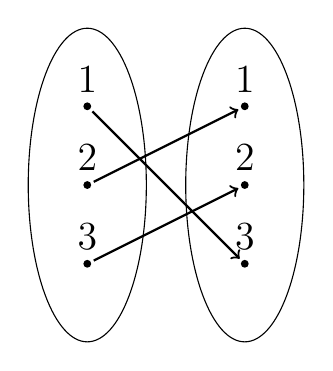
\begin{tikzpicture}[ele/.style={fill=black, circle, minimum width=.1pt, inner sep=1pt},every fit/.style={ellipse, draw, inner sep=10pt},every label/.append style={font=\Large}]
  \node[ele, label = above:$1$] (a1) at (0,4) {};
  \node[ele, label = above:$2$] (a2) at (0,3) {};
  \node[ele, label = above:$3$] (a3) at (0,2) {};

  \node[ele, label = above:$1$] (b1) at (2,4) {};
  \node[ele, label = above:$2$] (b2) at (2,3) {};
  \node[ele, label = above:$3$] (b3) at (2,2) {};

  \node[draw, fit = (a1) (a2) (a3), minimum width = 1.5cm] {};
  \node[draw, fit = (b1) (b2) (b3), minimum width = 1.5cm] {};
 
  \draw[->, thick, shorten <= 1pt, shorten >= 1pt] (a1) -- (b3);
  \draw[->, thick, shorten <= 1pt, shorten >= 1pt] (a2) -- (b1);
  \draw[->, thick, shorten <= 1pt, shorten >= 1pt] (a3) -- (b2);
 \end{tikzpicture}
\end{center}

\centerline{\LARGE \( \sigma^{2} \)}
\vspace{5mm}

\section{Finite Cyclic Groups}

Finite cyclic groups typically are denoted by \( C_{n}, \text{where} \: n \in \blackboard{N}\). They contain all the cyclic permutations of the set of natural numbers less than or equal to $n$.

A useful way to understand the finite cyclic groups is a wheel pinned at the centre with the numbers 1 to $n$ arranged clockwise around the edge, as seen below. The group $C_{n}$ corresponds to the set of permutations corresponding to rotations of the wheel.

For example $C_{9}$ corresponds to all the possible rotational states of the following circle:

\begin{center}
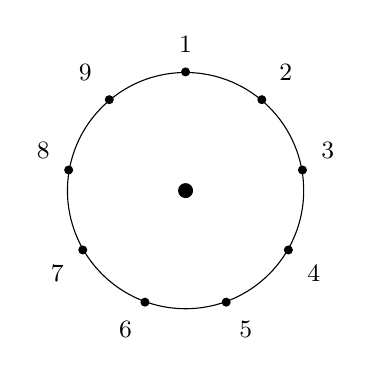
\begin{tikzpicture}

\drawvertices[
    num vertex=9, 
    circle radius=3,
    vertex radius=1pt,
    shift angle=90,
    circumference with labels in order={
    black,black,black,black,black,black,black,black,black
    }] {};
    
\draw[fill=black] circle (2.5pt);

\end{tikzpicture}
\end{center}

In general we have:

\[C_{n} = \{ i, \sigma, \sigma^{2}, ..., \sigma^{n-1} \}\]

The first two cyclic groups for $n=1,2$ are equivalent to the symmetric groups, the similarities end at $n=3$ however, with the group given as:

\[C_{3} = \{ i, \sigma, \sigma^{2} \}\]

with the following composition table:

\begin{center}
\begin{tabular}{ |c|c c c| } 
 \hline
 $\circ$ & i & $\sigma$ & $\sigma^{2}$ \\
 \hline
 i & i & $\sigma$ & $\sigma^{2}$ \\
 $\sigma$ & $\sigma$ & $\sigma^{2}$ & i \\
 $\sigma^{2}$ & $\sigma^{2}$ & i & $\sigma$ \\
 \hline
\end{tabular}
\end{center}

which corresponds to the set permutations defined in the symmetric group section.

\section{Dihedral Groups}

The dihedral groups are denoted by \( D_{n}, \text{where} \: n \in \blackboard{N}\). They contain all the permutations within the finite cyclic group, with the addition of permutations achieved by flipping the elements in a second axis. This can be best understood by considering all the possible permutations of a disk when the disk is rotated and when it is lifted off the 2D plane and flipped over. For example $D_{9}$ can be represented by the following circle below, which has no pin at the center.

\begin{center}
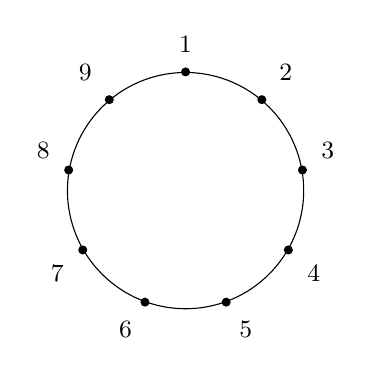
\begin{tikzpicture}

\drawvertices[
    num vertex=9, 
    circle radius=3,
    vertex radius=1pt,
    shift angle=90,
    circumference with labels in order={
    black,black,black,black,black,black,black,black,black
    }] {};

\end{tikzpicture}
\end{center}

The order of the dihedral group is given as:

\[ |D_{n}| = 2n \]

\end{document}


